For the circuit shown in Fig. \ref{fig:ee18btech11047_fig1}, find the loop gain $L(s) = G(s)H(s)$, $L(j\omega)$, the frequency for zero loop phase, and $R_{2}/R_{1}$ for oscillation.
\begin{enumerate}[label=\arabic*.,ref=\theenumi]
%\begin{enumerate}[label=\thesection.\arabic*.,ref=\thesection.\theenumi]
\numberwithin{equation}{enumi}

\item Draw the equivalent control system representation for the circuit in Fig. \ref{fig:ee18btech11047_fig1} as well as the small signal model.
\\
\solution See Figs. \ref{fig:ee18btech11047_fig2} and 


\renewcommand{\thefigure}{\theenumi.\arabic{figure}}
%
\begin{figure}[!ht]
	\begin{center}
		\resizebox{\columnwidth}{!}{\begin{circuitikz}
\ctikzset{bipoles/length=1cm}

 
\draw (0, 0) node[op amp] (opamp) {};
\draw (opamp.-) --(-1,0.35)-- (-1,1) to[R=$R_2$,*-*] (1,1) -- (1,0) -- (1,-1) to [C=$C$,*-*] (0.25,-1) to [R=$R$,*-*] (-1,-1) -- (-1,-0.35) to (opamp.+);
\draw (-1,1) to[R=$R_1$,*-*] (-3.5, 1) to node[ground]{}  (-3.5, 0.9) ;
\draw (0.25,-1) to [R = $R$,*-*] (0.25,-3) to node[ground]{} (0.25,-3);
\draw (-1,-1) to[C=$C$,*-*] (-1, -3) to node[ground]{} (-1,-3);
\draw (opamp.out) -- (1,0) ;
%node at (1.5,0){};
\end{circuitikz}

}
	\end{center}
\caption{}
\label{fig:ee18btech11047_fig1}
\end{figure}
%
\solution See Fig. \ref{fig:ee18btech11047_fig2}. Oscillators do not include input signal.
\begin{figure}[!ht]
	\begin{center}
		\resizebox{\columnwidth}{!}{%%%%%%%%%%%%%%%%%%%%%%%%%%%%%%%%%%%%%%%%%%%%%%%%%%%%%%%%%%%%%%%%%%%%%%
%%                                                                  %%
%%  This is the header of a LaTeX2e file exported from Gnumeric.    %%
%%                                                                  %%
%%  This file can be compiled as it stands or included in another   %%
%%  LaTeX document. The table is based on the longtable package so  %%
%%  the longtable options (headers, footers...) can be set in the   %%
%%  preamble section below (see PRAMBLE).                           %%
%%                                                                  %%
%%  To include the file in another, the following two lines must be %%
%%  in the including file:                                          %%
%%        \def\inputGnumericTable{}                                 %%
%%  at the beginning of the file and:                               %%
%%        \input{name-of-this-file.tex}                             %%
%%  where the table is to be placed. Note also that the including   %%
%%  file must use the following packages for the table to be        %%
%%  rendered correctly:                                             %%
%%    \usepackage[latin1]{inputenc}                                 %%
%%    \usepackage{color}                                            %%
%%    \usepackage{array}                                            %%
%%    \usepackage{longtable}                                        %%
%%    \usepackage{calc}                                             %%
%%    \usepackage{multirow}                                         %%
%%    \usepackage{hhline}                                           %%
%%    \usepackage{ifthen}                                           %%
%%  optionally (for landscape tables embedded in another document): %%
%%    \usepackage{lscape}                                           %%
%%                                                                  %%
%%%%%%%%%%%%%%%%%%%%%%%%%%%%%%%%%%%%%%%%%%%%%%%%%%%%%%%%%%%%%%%%%%%%%%



%%  This section checks if we are begin input into another file or  %%
%%  the file will be compiled alone. First use a macro taken from   %%
%%  the TeXbook ex 7.7 (suggestion of Han-Wen Nienhuys).            %%
\def\ifundefined#1{\expandafter\ifx\csname#1\endcsname\relax}


%%  Check for the \def token for inputed files. If it is not        %%
%%  defined, the file will be processed as a standalone and the     %%
%%  preamble will be used.                                          %%
\ifundefined{inputGnumericTable}

%%  We must be able to close or not the document at the end.        %%
	\def\gnumericTableEnd{\end{document}}


%%%%%%%%%%%%%%%%%%%%%%%%%%%%%%%%%%%%%%%%%%%%%%%%%%%%%%%%%%%%%%%%%%%%%%
%%                                                                  %%
%%  This is the PREAMBLE. Change these values to get the right      %%
%%  paper size and other niceties.                                  %%
%%                                                                  %%
%%%%%%%%%%%%%%%%%%%%%%%%%%%%%%%%%%%%%%%%%%%%%%%%%%%%%%%%%%%%%%%%%%%%%%

	\documentclass[12pt%
			  %,landscape%
                    ]{report}
       \usepackage[latin1]{inputenc}
       \usepackage{fullpage}
       \usepackage{color}
       \usepackage{array}
       \usepackage{longtable}
       \usepackage{calc}
       \usepackage{multirow}
       \usepackage{hhline}
       \usepackage{ifthen}

	\begin{document}


%%  End of the preamble for the standalone. The next section is for %%
%%  documents which are included into other LaTeX2e files.          %%
\else

%%  We are not a stand alone document. For a regular table, we will %%
%%  have no preamble and only define the closing to mean nothing.   %%
    \def\gnumericTableEnd{}

%%  If we want landscape mode in an embedded document, comment out  %%
%%  the line above and uncomment the two below. The table will      %%
%%  begin on a new page and run in landscape mode.                  %%
%       \def\gnumericTableEnd{\end{landscape}}
%       \begin{landscape}


%%  End of the else clause for this file being \input.              %%
\fi

%%%%%%%%%%%%%%%%%%%%%%%%%%%%%%%%%%%%%%%%%%%%%%%%%%%%%%%%%%%%%%%%%%%%%%
%%                                                                  %%
%%  The rest is the gnumeric table, except for the closing          %%
%%  statement. Changes below will alter the table's appearance.     %%
%%                                                                  %%
%%%%%%%%%%%%%%%%%%%%%%%%%%%%%%%%%%%%%%%%%%%%%%%%%%%%%%%%%%%%%%%%%%%%%%

\providecommand{\gnumericmathit}[1]{#1} 
%%  Uncomment the next line if you would like your numbers to be in %%
%%  italics if they are italizised in the gnumeric table.           %%
%\renewcommand{\gnumericmathit}[1]{\mathit{#1}}
\providecommand{\gnumericPB}[1]%
{\let\gnumericTemp=\\#1\let\\=\gnumericTemp\hspace{0pt}}
 \ifundefined{gnumericTableWidthDefined}
        \newlength{\gnumericTableWidth}
        \newlength{\gnumericTableWidthComplete}
        \newlength{\gnumericMultiRowLength}
        \global\def\gnumericTableWidthDefined{}
 \fi
%% The following setting protects this code from babel shorthands.  %%
 \ifthenelse{\isundefined{\languageshorthands}}{}{\languageshorthands{english}}
%%  The default table format retains the relative column widths of  %%
%%  gnumeric. They can easily be changed to c, r or l. In that case %%
%%  you may want to comment out the next line and uncomment the one %%
%%  thereafter                                                      %%
\providecommand\gnumbox{\makebox[0pt]}
%%\providecommand\gnumbox[1][]{\makebox}

%% to adjust positions in multirow situations                       %%
\setlength{\bigstrutjot}{\jot}
\setlength{\extrarowheight}{\doublerulesep}

%%  The \setlongtables command keeps column widths the same across  %%
%%  pages. Simply comment out next line for varying column widths.  %%
\setlongtables

\setlength\gnumericTableWidth{%
	53pt+%
	93pt+%
0pt}
\def\gumericNumCols{2}
\setlength\gnumericTableWidthComplete{\gnumericTableWidth+%
         \tabcolsep*\gumericNumCols*2+\arrayrulewidth*\gumericNumCols}
\ifthenelse{\lengthtest{\gnumericTableWidthComplete > \linewidth}}%
         {\def\gnumericScale{\ratio{\linewidth-%
                        \tabcolsep*\gumericNumCols*2-%
                        \arrayrulewidth*\gumericNumCols}%
{\gnumericTableWidth}}}%
{\def\gnumericScale{1}}

%%%%%%%%%%%%%%%%%%%%%%%%%%%%%%%%%%%%%%%%%%%%%%%%%%%%%%%%%%%%%%%%%%%%%%
%%                                                                  %%
%% The following are the widths of the various columns. We are      %%
%% defining them here because then they are easier to change.       %%
%% Depending on the cell formats we may use them more than once.    %%
%%                                                                  %%
%%%%%%%%%%%%%%%%%%%%%%%%%%%%%%%%%%%%%%%%%%%%%%%%%%%%%%%%%%%%%%%%%%%%%%

\ifthenelse{\isundefined{\gnumericColA}}{\newlength{\gnumericColA}}{}\settowidth{\gnumericColA}{\begin{tabular}{@{}p{90pt*\gnumericScale}@{}}x\end{tabular}}
\ifthenelse{\isundefined{\gnumericColB}}{\newlength{\gnumericColB}}{}\settowidth{\gnumericColB}{\begin{tabular}{@{}p{53pt*\gnumericScale}@{}}x\end{tabular}}

\begin{tabular}[c]{%
	b{\gnumericColA}%
	b{\gnumericColB}%
	}

%%%%%%%%%%%%%%%%%%%%%%%%%%%%%%%%%%%%%%%%%%%%%%%%%%%%%%%%%%%%%%%%%%%%%%
%%  The longtable options. (Caption, headers... see Goosens, p.124) %%
%	\caption{The Table Caption.}             \\	%
% \hline	% Across the top of the table.
%%  The rest of these options are table rows which are placed on    %%
%%  the first, last or every page. Use \multicolumn if you want.    %%

%%  Header for the first page.                                      %%
%	\multicolumn{2}{c}{The First Header} \\ \hline 
%	\multicolumn{1}{c}{colTag}	%Column 1
%	&\multicolumn{1}{c}{colTag}	\\ \hline %Last column
%	\endfirsthead

%%  The running header definition.                                  %%
%	\hline
%	\multicolumn{2}{l}{\ldots\small\slshape continued} \\ \hline
%	\multicolumn{1}{c}{colTag}	%Column 1
%	&\multicolumn{1}{c}{colTag}	\\ \hline %Last column
%	\endhead

%%  The running footer definition.                                  %%
%	\hline
%	\multicolumn{2}{r}{\small\slshape continued\ldots} \\
%	\endfoot

%%  The ending footer definition.                                   %%
%	\multicolumn{2}{c}{That's all folks} \\ \hline 
%	\endlastfoot
%%%%%%%%%%%%%%%%%%%%%%%%%%%%%%%%%%%%%%%%%%%%%%%%%%%%%%%%%%%%%%%%%%%%%%

\hhline{|-|-}
	 \multicolumn{1}{|p{\gnumericColA}|}%
	{\gnumericPB{\centering}\gnumbox{\textbf{Poles}}}
	&\multicolumn{1}{p{\gnumericColB}|}%
	{\gnumericPB{\centering}\gnumbox{\textbf{Zeros}}}
\\
\hhline{|--|}
	 \multicolumn{1}{|p{\gnumericColA}|}%
	{\gnumericPB{\centering}\gnumbox{$p_{1}=-0.72$}}
	&\multicolumn{1}{p{\gnumericColB}|}%
	{$z_{1}=-5$}
\\
\hhline{|--|}
	 \multicolumn{1}{|p{\gnumericColA}|}%
	{\gnumericPB{\centering}\gnumbox{$p_{2}=-7.64+6.75j$}}
	&\multicolumn{1}{p{\gnumericColB}|}%
	{}
\\
\hhline{|--|}
	 \multicolumn{1}{|p{\gnumericColA}|}%
	{\gnumericPB{\centering}\gnumbox{$p_{3}=-7.63-6.75j$}}
	&\multicolumn{1}{p{\gnumericColB}|}%
	{}
\\
\hhline{|-|-|}
\end{tabular}

\ifthenelse{\isundefined{\languageshorthands}}{}{\languageshorthands{\languagename}}
\gnumericTableEnd
}
	\end{center}
\caption{}
\label{fig:ee18btech11047_fig2}
\end{figure}
%
\begin{figure}[!ht]
	\begin{center}
		\resizebox{\columnwidth}{!}{\usetikzlibrary{decorations.markings}
\begin{circuitikz}
\ctikzset{bipoles/length=1cm}

\draw 
(1.5,1) to [C=$C$] (1.5,5) to (1.5,5)  node[ground,rotate=180]{} 
(1.5,2) to [R=$R$] (3.5,2) to [R=$R$,*-*] (3.5,4) to (3.5,5) node[ground,rotate=180]{} 
(3.5,2) to [C=$C$] (5,2) -- (5,1)
%(1.5,3) node[pos=10]{$V_i$}
(1.5,-1.25)  node at(1.7,-1.25){$-$} 
(1.5,-1.25) -- (1,-1.25) -- (1,-1.75) to[R=$R_1$] (1,-2.75) --(1,-3) node[ground]{}
(1,-1.5) to[R=$R_2$,*-*] (5,-1.5) {}
(5,-1.5) -- (5,1) --(3.5,1) to[V=$G_{1}V_i$] (3.5,-0.5) node[ground]{}
(5,1) --(6,1)
(6,1) --(6.5,1) node at(6.8,1){$V_o$}
node at (1.8,-0.3) {$V_i$}
node at (3.5,1.7) {$V_{a}$}
node at (1.1,2) {$V_{f}$}
node at(1.8,1){$+$}
;\end{circuitikz}
}
	\end{center}
\caption{}
\label{fig:ee18btech11047_fig3}
\end{figure}
\renewcommand{\thefigure}{\theenumi}
%
\item Find the open loop gain $G$.\\
\label{prob:ee18btech11047_G}
\solution Let the closed loop gain, open-loop gain of op-amp connected in non-inverting configuration be $T_{1}$ and $G_{1}$ respectively.
From Table \ref{table:ee18btech11005_Output_Table}
\begin{align}
T_{1} &= \frac{G_{1}\brak{R_1+R_2}}{\brak{R_1+R_2}+G_{1}R_1}
\end{align}
\begin{align}
T_{1} &= \frac{\brak{R_1+R_2}}{\brak{R_1+R_2}/G_{1}+R_1}
\end{align}
Assuming $G_{1}\to\infty$
\begin{align}
T_{1} &= 1 + \frac{R_{2}}{R_{1}}
\end{align}
The open loop gain of the circuit shown in Fig. \ref{fig:ee18btech11047_fig1} is equal to the closed loop gain of an op-amp connected in non-inverting configuration.
\begin{align}
G &= T_{1}
\end{align}
\begin{align}
\label{eq:ee18btech11047_1}
\implies G = 1 + \frac{R_{2}}{R_{1}}
\end{align}
%
\item Find the feedback factor $H$. \\
\label{prob:ee18btech11047_H}
\solution The small signal model is shown in Fig. \ref{fig:ee18btech11047_fig3}
Applying KCL at node $V_f$
\begin{align}
\frac{V_{f} - 0}{\frac{1}{sC}} +\frac{V_{f} - V_{a}}{R} &= 0
\end{align}
\begin{align}
V_{f}\brak{sC+\frac{1}{R}} &= \frac{V_{a}}{R} 
\end{align}
\begin{align}
\label{eq:ee18btech11047_2}
V_{a} &= V_{f}\brak{sRC + 1} 
\end{align}
Applying KCL at node $V_{a}$
\begin{align}
\frac{V_{a} - V_{f}}{R} + \frac{V_{a} - 0}{R} + \frac{V_{a} - V_{o}}{\frac{1}{sC}} &= 0
\end{align}
\begin{align}
V_{a}\brak{\frac{2}{R} +sC} &= \frac{V_{f}}{R} + V_{o}sC
\end{align}
Substitute $V_{a}$ value from equation\eqref{eq:ee18btech11047_2}
\begin{align}
V_{f}(sRC + 1)\brak{\frac{2}{R} + sC} &= \frac{V_{f}}{R} + V_{o}sC
\end{align}
\begin{align}
V_{f}\brak{3 + sRC + \frac{1}{sRC}} &= V_{o}
\end{align}
The feedback factor H is given by 
\begin{align}
H &= \frac{V_{f}}{V_{o}}
\end{align}
\begin{align}
\label{eq:ee18btech11047_3}
\implies H &= \frac{1}{\brak{3+sRC +\frac{1}{sRC}}}
\end{align}
%
\item Find the loop gain L(s).\\
\solution The transfer function of the equivalent positive feedback circuit in Fig. \ref{fig:ee18btech11047_fig2} is  
\begin{align}
T &= \frac{G}{1-GH}
\label{eq:ee18btech11047_TF}
\end{align}
Therefore, loop gain is given by 
\begin{align}
L &= GH
\end{align}
From equations \eqref{eq:ee18btech11047_1} and \eqref{eq:ee18btech11047_3}
\begin{align}
L(s) &= \brak{1 + \frac{R_{2}}{R_{1}}}\brak{\frac{1}{3+sRC+\frac{1}{sRC}}}
\end{align}
\begin{align}
\label{eq:ee18btech11047_4}
\implies L(s) &= \brak{\frac{1+\frac{R_{2}}{R_{1}}}{3+sRC+\frac{1}{sRC}}}
\end{align}
%
\item Find the loop gain in terms of $j\omega$ .\\
\solution Substitute $s = j\omega$ in equation \eqref{eq:ee18btech11047_4}
\begin{align} 
L(j\omega)&= \brak{\frac{1+\frac{R_{2}}{R_{1}}}{3+j\omega RC+\frac{1}{j\omega RC}}}
\end{align}
\begin{align}
\label{eq:ee18btech11047_5}
\implies L(j\omega)&= \brak{\frac{1+\frac{R_{2}}{R_{1}}}{3+ j \brak{\omega RC-\frac{1}{\omega RC}}}}
\end{align}
\item Find the frequency for zero loop phase.\\
\solution The frequency at which loop phase will be zero (i.e. loop gain will be a real number).To obtain the required frequency, equate the imaginary part of the loop gain $L(j \omega )$ to zero.
\begin{align}
j\brak{\omega RC - \frac{1}{\omega RC}} &= 0
\end{align}
\begin{align}
\omega^{2} &= \frac{1}{(RC)^{2}}
\end{align}
\begin{align}
\label{eq:ee18btech11047_freq}
\implies \omega &= \frac{1}{RC}
\end{align}
%
\item Find $R_{2}/R_{1}$ for oscillation.\\
\solution For oscillations to start, 
\begin{itemize}
    \item the imaginary part of the loop gain should become zero.
    \item the loop gain must be at least equal to unity.
\end{itemize}
From equation \eqref{eq:ee18btech11047_5} 
\begin{align}
\brak{\frac{1+\frac{R_{2}}{R_{1}}}{3+j(0)}} &\geq 1
\end{align}
\begin{align}
1+\frac{R_{2}}{R_{1}} &\geq 3
\end{align}
\begin{align}
\implies \frac{R_{2}}{R_{1}} &\geq 2
\end{align}
%----------------------------------------------------
\item Draw the block diagram and circuit diagram for $H$.\\
\renewcommand{\thefigure}{\theenumi.\arabic{figure}}
\begin{figure}[!ht]
	\begin{center}
		\resizebox{\columnwidth}{!}{\begin{circuitikz}[american]
\usetikzlibrary{positioning, fit, calc}
\draw (0,0)to [open,v=$V_f$]++(0,-2)to[short]++(6,0)
(0,0)to++(6,0);
\draw (8,-1)node[draw,minimum width=4cm,minimum height=4cm] (load) {H}(8,0)
(10,0)--++(6,0)
(10,-2)--(16,-2)
node at (16,-1.7) {$-$}
node at (16,-0.3){$+$}
node at (16,-1){$V_o$}
;
\end{circuitikz}
}
	\end{center}
\caption{Feedback block diagram}
\label{fig:ee18btech11047_fig4}
\end{figure}
\begin{figure}[!ht]
	\begin{center}
		\resizebox{\columnwidth}{!}{\begin{circuitikz}
\ctikzset{bipoles/length=1cm}

\draw (0,0) to [R=$R$,*-*] (2,0) to [C=$C$,*-*] (3,0);
\draw (0.5,0) to [C=$C$](0.5,-2) to node[ground]{} (0.5,-2);
\draw (2,0) to [R=$R$](2,-2) to node[ground]{} (2,-2);
\draw node at (-0.3,0) {$V_f$};
\draw node at (3.3,0) {$V_o$};
\end{circuitikz}
}
	\end{center}
\caption{Feedback circuit}
\label{fig:ee18btech11047_fig5}
\end{figure}
\renewcommand{\thefigure}{\theenumi}
\solution See figs \ref{fig:ee18btech11047_fig4} and \ref{fig:ee18btech11047_fig5} .From Fig. \ref{fig:ee18btech11047_fig5},the analysis is same as problem \ref{prob:ee18btech11047_H}
\begin{align}
\frac{V_{f}}{V_{o}} &= \frac{1}{\brak{3+sRC +\frac{1}{sRC}}}
\end{align}
\begin{align}
\implies H &= \frac{1}{\brak{3+sRC +\frac{1}{sRC}}}
\end{align}
%
\item Find the input and output resistances of the feedback network.\\
\solution To find the input resistance $R_{11}$ short the output node $V_{o}$ to ground.
\begin{align}
R_{11} &= Z ||(R+ (R||Z)) 
\end{align}
where $Z=\frac{1}{sC}$ is the impedance of the capacitor.
\begin{align}
\label{eq:ee18btech11047_6}
\implies R_{11} &= \brak{\frac{1}{sC}||\brak{R+R ||\frac{1}{sC}}}
\end{align}
To find the output resistance $R_{22}$ short the input node $V_{f}$ to ground.
\begin{align}
R_{22} &= Z + (R||R)
\end{align}
\begin{align}
\implies R_{22} &= \frac{1}{sC} + \frac{R}{2}   
\end{align}
%
\item Draw the block diagram and circuit diagram for $G$.\\
\renewcommand{\thefigure}{\theenumi.\arabic{figure}}
%
\begin{figure}[!ht]
	\begin{center}
		\resizebox{\columnwidth}{!}{\begin{circuitikz}[american]
\usetikzlibrary{positioning, fit, calc}
\draw (0,0)to [open,v=$V_i$]++(0,-2)to[short]++(6,0)
(0,0)to++(6,0);
\draw (8,-1)node[draw,minimum width=4cm,minimum height=4cm] (load) {G}(8,0)
(10,0) -- (16,0)
(3,0) to [R=$R_{11}$](3,-2)
(10,-2) to [R=$R_{22}$](16,-2)
node at (16,-1.7) {$-$}
node at (16,-0.3){$+$}
node at (16,-1){$V_o$}
;
\end{circuitikz}
}
	\end{center}
\caption{Open loop block diagram}
\label{fig:ee18btech11047_fig6}
\end{figure}
%
\begin{figure}[!ht]
	\begin{center}
		\resizebox{\columnwidth}{!}{\usetikzlibrary{decorations.markings}
\begin{circuitikz}
\ctikzset{bipoles/length=1cm}

\draw 
(1.5,1) to [C=$C$] (1.5,5) to (1.5,5)  node[ground,rotate=180]{} 
(1.5,2) to [R=$R$] (3,2) to [R=$R$] (3,4) to (3,5) node[ground,rotate=180]{} 
(3,2) --  (4.5,2) to [C=$C$](4.5,4) to (4.5,5) node[ground,rotate=180]{}
%(1.5,3) node[pos=10]{$V_i$}
(1.5,-1.25)  node at(1.7,-1.25){$-$} 
(1.5,-1.25) -- (1,-1.25) -- (1,-1.75) to[R=$R_1$] (1,-2.75) --(1,-3) node[ground]{}
(1,-1.5) to[R=$R_2$,*-*] (5,-1.5) {}
(5,-1.5) -- (5,1) --(3.5,1) to[V=$G_{1}V_i$] (3.5,-0.5) node[ground]{}
(5,1) --(6,1)
(6,1) --(7,1) node at(7.3,1){$V_o$}
(6,1) to [C=$C$](6,-0.5) to [R=$R$] (6,-2) to (6,-2) node[ground]{} 
(6,-0.5) -- (6.8,-0.5) to [R=$R$] (6.8,-2) to (6.8,-2) node[ground]{}
node at (1.8,-0.3) {$V_i$}  
node at (1.1,2) {$V_{f}$}
node at(1.8,1){$+$}
;\end{circuitikz}
}
	\end{center}
\caption{Open loop circuit diagram}
\label{fig:ee18btech11047_fig7}
\end{figure}
\renewcommand{\thefigure}{\theenumi}
\solution See figs \ref{fig:ee18btech11047_fig6} and \ref{fig:ee18btech11047_fig7}.From Fig. \ref{fig:ee18btech11047_fig7} using same analysis as problem \ref{prob:ee18btech11047_G}
\begin{align}
G &= \frac{V_{o}}{V_{i}}
\end{align}
\begin{align}
G &= \frac{R_{1} + R_{2}}{R_{1}}
\end{align}
\begin{align}
\implies G &= 1+\frac{R_{2}}{R_{1}}
\end{align}
Hence verified with equation \eqref{eq:ee18btech11047_1}.
\item Find the amplitude and frequency for some arbitrary values given in Table \ref{table:ee18btech110047_Input_Table}.\\
\begin{table}[!ht]
\centering
%%%%%%%%%%%%%%%%%%%%%%%%%%%%%%%%%%%%%%%%%%%%%%%%%%%%%%%%%%%%%%%%%%%%%%
%%                                                                  %%
%%  This is the header of a LaTeX2e file exported from Gnumeric.    %%
%%                                                                  %%
%%  This file can be compiled as it stands or included in another   %%
%%  LaTeX document. The table is based on the longtable package so  %%
%%  the longtable options (headers, footers...) can be set in the   %%
%%  preamble section below (see PRAMBLE).                           %%
%%                                                                  %%
%%  To include the file in another, the following two lines must be %%
%%  in the including file:                                          %%
%%        \def\inputGnumericTable{}                                 %%
%%  at the beginning of the file and:                               %%
%%        \input{name-of-this-file.tex}                             %%
%%  where the table is to be placed. Note also that the including   %%
%%  file must use the following packages for the table to be        %%
%%  rendered correctly:                                             %%
%%    \usepackage[latin1]{inputenc}                                 %%
%%    \usepackage{color}                                            %%
%%    \usepackage{array}                                            %%
%%    \usepackage{longtable}                                        %%
%%    \usepackage{calc}                                             %%
%%    \usepackage{multirow}                                         %%
%%    \usepackage{hhline}                                           %%
%%    \usepackage{ifthen}                                           %%
%%  optionally (for landscape tables embedded in another document): %%
%%    \usepackage{lscape}                                           %%
%%                                                                  %%
%%%%%%%%%%%%%%%%%%%%%%%%%%%%%%%%%%%%%%%%%%%%%%%%%%%%%%%%%%%%%%%%%%%%%%



%%  This section checks if we are begin input into another file or  %%
%%  the file will be compiled alone. First use a macro taken from   %%
%%  the TeXbook ex 7.7 (suggestion of Han-Wen Nienhuys).            %%
\def\ifundefined#1{\expandafter\ifx\csname#1\endcsname\relax}


%%  Check for the \def token for inputed files. If it is not        %%
%%  defined, the file will be processed as a standalone and the     %%
%%  preamble will be used.                                          %%
\ifundefined{inputGnumericTable}

%%  We must be able to close or not the document at the end.        %%
	\def\gnumericTableEnd{\end{document}}


%%%%%%%%%%%%%%%%%%%%%%%%%%%%%%%%%%%%%%%%%%%%%%%%%%%%%%%%%%%%%%%%%%%%%%
%%                                                                  %%
%%  This is the PREAMBLE. Change these values to get the right      %%
%%  paper size and other niceties.                                  %%
%%                                                                  %%
%%%%%%%%%%%%%%%%%%%%%%%%%%%%%%%%%%%%%%%%%%%%%%%%%%%%%%%%%%%%%%%%%%%%%%

	\documentclass[12pt%
			  %,landscape%
                    ]{report}
       \usepackage[latin1]{inputenc}
       \usepackage{fullpage}
       \usepackage{color}
       \usepackage{array}
       \usepackage{longtable}
       \usepackage{calc}
       \usepackage{multirow}
       \usepackage{hhline}
       \usepackage{ifthen}

	\begin{document}


%%  End of the preamble for the standalone. The next section is for %%
%%  documents which are included into other LaTeX2e files.          %%
\else

%%  We are not a stand alone document. For a regular table, we will %%
%%  have no preamble and only define the closing to mean nothing.   %%
    \def\gnumericTableEnd{}

%%  If we want landscape mode in an embedded document, comment out  %%
%%  the line above and uncomment the two below. The table will      %%
%%  begin on a new page and run in landscape mode.                  %%
%       \def\gnumericTableEnd{\end{landscape}}
%       \begin{landscape}


%%  End of the else clause for this file being \input.              %%
\fi

%%%%%%%%%%%%%%%%%%%%%%%%%%%%%%%%%%%%%%%%%%%%%%%%%%%%%%%%%%%%%%%%%%%%%%
%%                                                                  %%
%%  The rest is the gnumeric table, except for the closing          %%
%%  statement. Changes below will alter the table's appearance.     %%
%%                                                                  %%
%%%%%%%%%%%%%%%%%%%%%%%%%%%%%%%%%%%%%%%%%%%%%%%%%%%%%%%%%%%%%%%%%%%%%%

\providecommand{\gnumericmathit}[1]{#1} 
%%  Uncomment the next line if you would like your numbers to be in %%
%%  italics if they are italizised in the gnumeric table.           %%
%\renewcommand{\gnumericmathit}[1]{\mathit{#1}}
\providecommand{\gnumericPB}[1]%
{\let\gnumericTemp=\\#1\let\\=\gnumericTemp\hspace{0pt}}
 \ifundefined{gnumericTableWidthDefined}
        \newlength{\gnumericTableWidth}
        \newlength{\gnumericTableWidthComplete}
        \newlength{\gnumericMultiRowLength}
        \global\def\gnumericTableWidthDefined{}
 \fi
%% The following setting protects this code from babel shorthands.  %%
 \ifthenelse{\isundefined{\languageshorthands}}{}{\languageshorthands{english}}
%%  The default table format retains the relative column widths of  %%
%%  gnumeric. They can easily be changed to c, r or l. In that case %%
%%  you may want to comment out the next line and uncomment the one %%
%%  thereafter                                                      %%
\providecommand\gnumbox{\makebox[0pt]}
%%\providecommand\gnumbox[1][]{\makebox}

%% to adjust positions in multirow situations                       %%
\setlength{\bigstrutjot}{\jot}
\setlength{\extrarowheight}{\doublerulesep}

%%  The \setlongtables command keeps column widths the same across  %%
%%  pages. Simply comment out next line for varying column widths.  %%
\setlongtables

\setlength\gnumericTableWidth{%
	53pt+%
	93pt+%
0pt}
\def\gumericNumCols{2}
\setlength\gnumericTableWidthComplete{\gnumericTableWidth+%
         \tabcolsep*\gumericNumCols*2+\arrayrulewidth*\gumericNumCols}
\ifthenelse{\lengthtest{\gnumericTableWidthComplete > \linewidth}}%
         {\def\gnumericScale{\ratio{\linewidth-%
                        \tabcolsep*\gumericNumCols*2-%
                        \arrayrulewidth*\gumericNumCols}%
{\gnumericTableWidth}}}%
{\def\gnumericScale{1}}

%%%%%%%%%%%%%%%%%%%%%%%%%%%%%%%%%%%%%%%%%%%%%%%%%%%%%%%%%%%%%%%%%%%%%%
%%                                                                  %%
%% The following are the widths of the various columns. We are      %%
%% defining them here because then they are easier to change.       %%
%% Depending on the cell formats we may use them more than once.    %%
%%                                                                  %%
%%%%%%%%%%%%%%%%%%%%%%%%%%%%%%%%%%%%%%%%%%%%%%%%%%%%%%%%%%%%%%%%%%%%%%

\ifthenelse{\isundefined{\gnumericColA}}{\newlength{\gnumericColA}}{}\settowidth{\gnumericColA}{\begin{tabular}{@{}p{53pt*\gnumericScale}@{}}x\end{tabular}}
\ifthenelse{\isundefined{\gnumericColB}}{\newlength{\gnumericColB}}{}\settowidth{\gnumericColB}{\begin{tabular}{@{}p{93pt*\gnumericScale}@{}}x\end{tabular}}

\begin{tabular}[c]{%
	b{\gnumericColA}%
	b{\gnumericColB}%
	}

%%%%%%%%%%%%%%%%%%%%%%%%%%%%%%%%%%%%%%%%%%%%%%%%%%%%%%%%%%%%%%%%%%%%%%
%%  The longtable options. (Caption, headers... see Goosens, p.124) %%
%	\caption{The Table Caption.}             \\	%
% \hline	% Across the top of the table.
%%  The rest of these options are table rows which are placed on    %%
%%  the first, last or every page. Use \multicolumn if you want.    %%

%%  Header for the first page.                                      %%
%	\multicolumn{2}{c}{The First Header} \\ \hline 
%	\multicolumn{1}{c}{colTag}	%Column 1
%	&\multicolumn{1}{c}{colTag}	\\ \hline %Last column
%	\endfirsthead

%%  The running header definition.                                  %%
%	\hline
%	\multicolumn{2}{l}{\ldots\small\slshape continued} \\ \hline
%	\multicolumn{1}{c}{colTag}	%Column 1
%	&\multicolumn{1}{c}{colTag}	\\ \hline %Last column
%	\endhead

%%  The running footer definition.                                  %%
%	\hline
%	\multicolumn{2}{r}{\small\slshape continued\ldots} \\
%	\endfoot

%%  The ending footer definition.                                   %%
%	\multicolumn{2}{c}{That's all folks} \\ \hline 
%	\endlastfoot
%%%%%%%%%%%%%%%%%%%%%%%%%%%%%%%%%%%%%%%%%%%%%%%%%%%%%%%%%%%%%%%%%%%%%%

\hhline{|-|-}
	 \multicolumn{1}{|p{\gnumericColA}|}%
	{\gnumericPB{\centering}\gnumbox{\textbf{Parameter}}}
	&\multicolumn{1}{p{\gnumericColB}|}%
	{\gnumericPB{\centering}\gnumbox{\textbf{Value}}}
\\
\hhline{|--|}
	 \multicolumn{1}{|p{\gnumericColA}|}%
	{\gnumericPB{\centering}\gnumbox{$R$}}
	&\multicolumn{1}{p{\gnumericColB}|}%
	{$250 \Omega$}
\\
\hhline{|--|}
	 \multicolumn{1}{|p{\gnumericColA}|}%
	{\gnumericPB{\centering}\gnumbox{$C$}}
	&\multicolumn{1}{p{\gnumericColB}|}%
	{$1mF$}
\\
\hhline{|-|-|}
	 \multicolumn{1}{|p{\gnumericColA}|}%
	{\gnumericPB{\centering}\gnumbox{$R_{2}$}}
	&\multicolumn{1}{p{\gnumericColB}|}%
	{$2k\Omega $}
\\
\hhline{|--|}
	 \multicolumn{1}{|p{\gnumericColA}|}%
	{\gnumericPB{\centering}\gnumbox{$R_{1}$}}
	&\multicolumn{1}{p{\gnumericColB}|}%
	{$1k\Omega $}	
\\
\hhline{|-|-|}
\end{tabular}

\ifthenelse{\isundefined{\languageshorthands}}{}{\languageshorthands{\languagename}}
\gnumericTableEnd

\caption{}
\label{table:ee18btech110047_Input_Table}
\end{table}
\solution From equation \eqref{eq:ee18btech11047_1} 
\begin{align}
G &= 1 + \frac{R_{2}}{R_{1}} = 3
\end{align}
From equation \eqref{eq:ee18btech11047_3}
\begin{align}
H &= \frac{1}{3 + 0.25s + \frac{1}{0.25s}}
\end{align}
From equation \eqref{eq:ee18btech11047_TF}
\begin{align}
T &= \frac{3\brak{0.0625s^{2} + 0.75s + 1}}{0.0625s^{2} + 1}
\end{align}
The following code plots the oscillating response of the system.
\begin{lstlisting}
codes/ee18btech11047/ee18btech11047.py
\end{lstlisting}
\begin{figure}[!ht]
\centering
\includegraphics[width=\columnwidth]{./figs/ee18btech11047/ee18btech11047.eps}
\caption{}
\label{fig:ee18btech11047_fig8}
\end{figure}
\textbf{Amplitude:}From Fig. \ref{fig:ee18btech11047_fig8} V(peak-peak) is 
\begin{align}
V_{p-p} &= 18.12
\end{align}
\begin{align}
V_{max} &= \frac{V_{p-p}}{2} = 9.06
\end{align}
\textbf{Frequency:} From equation \eqref{eq:ee18btech11047_freq}
\begin{align}
\omega = \frac{1}{RC} = 4 rad/sec
\end{align}
\begin{align}
f = \frac{\omega }{2\pi} = 0.636 Hz
\end{align}
\end{enumerate}
